\documentclass{standalone}
\usepackage[svgnames]{xcolor}
\usepackage{tikz}

\begin{document}
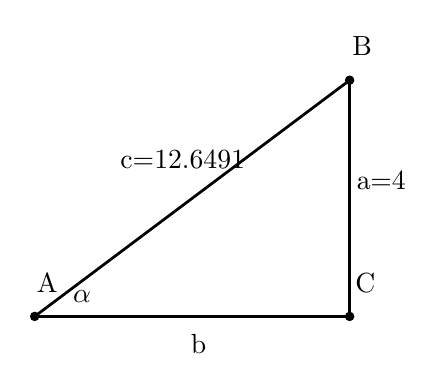
\begin{tikzpicture}
\draw [shift={(0,0)},line width=1pt] (0,0) -- (0:0.6);
\draw [line width=1pt] (0,0)-- (4,0);
\draw [line width=1pt] (4,0)-- (4,3);
\draw [line width=1pt] (4,3)-- (0,0);
\draw [fill=black] (0,0) circle (1.5pt);
\draw [fill=black] (4,0) circle (1.5pt);
\draw [fill=black] (4,3) circle (1.5pt);
\draw[color=black] (0.16,0.43) node {A};
\draw[color=black] (4.16,3.43) node {B};
\draw[color=black] (4.2,0.43) node {C};
\draw[color=black] (4.4,1.73) node {a=4};
\draw[color=black] (2.08,-0.35) node {b};
\draw[color=black] (1.88,1.99) node {c=12.6491};
\draw[color=black] (0.6,0.25) node {\(\alpha\)};
\end{tikzpicture}


\end{document}
